\documentclass{article}
\usepackage{amsmath,amsthm,amsfonts, amssymb}
\usepackage{hyperref}
\usepackage{tikz}
\usetikzlibrary{arrows,automata}
\usetikzlibrary{decorations.text,calc}

\setlength{\textheight}{8.5in}
\setlength{\evensidemargin}{0.0in}
\setlength{\oddsidemargin}{0.0in}
\setlength{\topmargin}{-0.5in}
\setlength{\textwidth}{6.5in}

\usepackage{prooftree}
\usepackage{boxproof}
\usepackage{parskip}

\newcommand{\handout}[6]{
   \renewcommand{\thepage}{#1-\arabic{page}}
   \noindent
   \begin{center}
      \vbox{
    \hbox to \textwidth { #2 \hfill #3 }
       \vspace{4mm}
       \hbox to \textwidth { {\Large \hfill #4  \hfill} }
       \vspace{4mm}
       \hbox to \textwidth { { #5 \hfill #6} }
      }
   \hrulefill
   \end{center}
   \vspace*{4mm}
}
\begin{document}
\handout{}{CS 512: Formal Methods}{Spring 2016}{Assignment 7: Modeling with LTL}{Instructor: Assaf Kfoury}{Author: Patrick Gomes}
\section{Problem 1}
a) \\

\begin{tikzpicture}
\tikzset{vertex/.style = {shape=circle,draw,minimum size=1.5em}}
\tikzset{edge/.style = {->,> = latex'}}

%vertices
\node[initial, vertex] (a) at (4,0) {S[P,Q,0]};
\node[vertex] (b) at (2, 2) {S[P,Q,1]};
\node[vertex] (c) at (6, 2) {S[P,Q,2]};
\node[vertex] (d) at (4, -2.5) {S[P,Q,-1]};
\node[vertex] (e) at (6.5, -2.5) {S[P,Q,-2]};
\node[vertex] (f) at (9,0) {S[P,0]};
\node[vertex] (g) at (8, 2) {S[P,1]};
\node[vertex] (h) at (10, 2) {S[P,2]};

%edges
%\draw[edge] (a) to[bend right] (b);
\draw[edge] (a) edge [bend right] node [below]{a} (b);
\draw[edge] (b) edge [bend right] node [above]{b} (a);
\draw[edge] (b) edge [bend left] node [above]{a} (c);
\draw[edge] (c) edge [bend right] node [above]{r} (a);
\draw[edge] (a) edge [bend right] node [left]{b} (d);
\draw[edge] (d) edge [bend right] node [right]{a} (a);
\draw[edge] (d) edge [bend right] node [below]{b} (e);
\draw[edge] (e) edge [bend right] node [below]{t} (f);
\draw[edge] (f) edge [bend left] node [below]{a} (g);
\draw[edge] (g) edge [bend left] node [above]{a} (h);
\draw[edge] (h) edge [bend left] node [right]{r} (f);


\end{tikzpicture}
\\
b) \\
\begin{align*}
	\text{E\{P,Q,1\} = ab + aar}\\
	\text{E\{P,Q,2\} = aar}\\
	\text{E\{P,Q,-1\} = ba}\\
	\text{Combining these all gives you E = (ab + aar + ba)*}
\end{align*}

c)\\
\begin{align*}
	\text{The path (bbt) brings us to S[P,0] and then repeat (aar) infinitely.}\\
	\text{Thus F = E + bbt + (aar)$^w$}
\end{align*}

d)\\
\begin{align*}
	\text{L(S[P,Q,0]) = \{a $\lor$ b $\lor$ r\}}\\
	\text{L(S[P,Q,1]) = \{a\}}\\
	\text{L(S[P,Q,2]) = \{a\}}\\
	\text{L(S[P,Q,-1]) = \{b\}}\\
	\text{L(S[P,Q,-2]) = \{b\}}\\
	\text{L(S[P,0]) = \{r $\lor$ t\}}\\
	\text{L(S[P,1]) = \{a\}}\\
	\text{L(S[P,2]) = \{a\}}\\
\end{align*}

e)\\
\begin{align*}
	\varphi_1 \triangleq G\ F\ r\\
	\text{Path for }\varphi_1 = b, b, t, (a,a,r)^*\\
	\mathcal{M} \nvDash \varphi_1, \text{an infinite path (a,b)$^*$ will never make r true at any point.}
\end{align*}
\begin{align*}
	\varphi_2 \triangleq G ((r \lor t) \to (Xa \land XX a))\\
	\text{Path for }\varphi_2 = b, b, t, (a,a,r)^*\\
	\mathcal{M} \nvDash \varphi_2, \text{an infinite path (a,a,r,b,a)* will not satisfy the conditional statement ever.}
\end{align*}
\begin{align*}
	\varphi_3 \triangleq ((a \lor b \lor r)\ U\ t)\\
	\text{Path for } \varphi_3 = b,b,t, (a,a,r)^*\\
	\mathcal{M} \nvDash \varphi_3, \text{an infinite path (a,b)$^*$ will never make t true at any point, so the strong until is never met.}
\end{align*}

\section{Problem 2}
\begin{align*}
	\text{The conditions from the book:}\\
	\phi\ is\ a\ literal: return\ \phi \\
	\phi\ is\ \neg \neg \phi_1: return\ \text{NNF}(\phi_1)\\
	\phi\ is\ \phi_1 \land \phi_2: return\ \text{NNF}(\phi_1) \land \text{NNF}(\phi_2)\\
	\phi\ is\ \phi_1 \lor \phi_2: return\ \text{NNF}(\phi_1) \lor \text{NNF}(\phi_2)\\
	\phi\ is\ \neg(\phi_1 \land \phi_2): return\ \text{NNF}(\neg \phi_1) \lor \text{NNF}(\neg \phi_2)\\
	\phi\ is\ \neg(\phi_1 \lor \phi_2): return\ \text{NNF}(\neg \phi_1) \land \text{NNF}(\neg\phi_2)\\
	\text{On top of all of these conditions, you need to add the following conditions:}\\
	\phi\ is\ X\phi_1: return\ X \text{NNF}(\phi_1)\\
	\phi\ is\ \neg X\phi_1: return\ \neg X\ \text{NNF}(\phi_1)\\
	\phi\ is\ F\phi_1: return\ F\ \text{NNF}(\phi_1)\\
	\phi\ is\ \neg F\phi_1: return\ G\ \text{NNF}(\neg \phi_1)\\
	\phi\ is\ G\phi_1: return\ G\ \text{NNF}(\phi_1)\\
	\phi\ is\ \neg G\phi_1: return\ F\ \text{NNF}(\neg \phi_1)\\
	\phi\ is\ \phi_1 U \phi_2: return\ \text{NNF}(\phi_1)\ U\ \text{NNF}(\phi_2)\\
	\phi\ is\ \neg(\phi_1 U \phi_2): return\ \text{NNF}(\neg \phi_1)\ R\ \text{NNF}(\neg \phi_2)\\
	\phi\ is\ \phi_1 R \phi_2: return\ \text{NNF}(\phi_1)\ R\ \text{NNF}(\phi_2)\\
	\phi\ is\ \neg(\phi_1 R \phi_2): return\ \text{NNF}(\neg \phi_1)\ U\ \text{NNF}(\neg \phi_2)\\
	\phi\ is\ \phi_1 W \phi_2: return\ \text{NNF}(\phi_1)\ W\ \text{NNF}(\phi_2)\\
	\phi\ is\ \neg(\phi_1 R \phi_2): return\ \text{NNF}(\neg(\phi_2\ R\ (\phi_1 \lor \phi_2)))\\
\end{align*}

\end{document}